\section{Language-Independent Smell Detection}~\label{sec:approach}

This section resolves 2 questions: 1. what are the definitions of the code
smells that \texttt{TreeNose} detects, and 2. what's the approach that
\texttt{TreeNose} uses to detect code smells across multiple programming
languages.

\subsection{Definitions of the Selected Code Smells}~\label{sec:definitions}

Code smells was first defined by Folwer and Beck back to 1999 in their book \textit{Refactoring},
where they defined 22 kinds of code smells \cite{Fowler_Beck}. Sine then, many researchers dedicated to define more
code smells and to improve the existing ones. This paper will focus on the code smells that are top 15 most common in
an empirical study conducted by Yamashita \& Moonen \cite{developersCare}.
Among them, we selected 5 code smells that occur across multiple programming languages: 1. Complex Conditional, 2. Long Class,
3. Long Method, 4. Long Parameter List, and 5. Long Message Chain. The definitions of these code smells are as follows:

\textbf{Complex Conditional (CC)} \cite{Fowler_Beck}: this smell occur when a conditional clause contains too many conditions,
such as nested if-else statements, and enormous switch-case statements. This smell makes the code hard to read and maintain on logic level.

\textbf{Long Class (LC)} \cite{Fowler_Beck}: a class handles too much work. Normally it occurs with too many properties. Or a class has too many lines because of
the extremely long properties.

\textbf{Long Method (LM)} \cite{Fowler_Beck}: a method grows too long. Normally it occurs with too many lines of code. The longer a method is, the harder it is to understand the procedure.

\textbf{Long Message Chain (LMC)} \cite{Fowler_Beck}: a long chain of object calls. This smell occurs when a method or an attribute calls another method or an attribute, and so on.

\textbf{Long Parameter List (LPL)} \cite{Fowler_Beck}: a method or a function has too many parameters. When a method has too many parameters, it often indicates that the method is doing too much work.

\begin{figure}[t]
    % Figures should be centered in the page/column
    \centering
    %
    \vspace*{-1em}
    %
    % Figure content goes here. This could be a graphic,
    % a TikZ diagram, etc.
    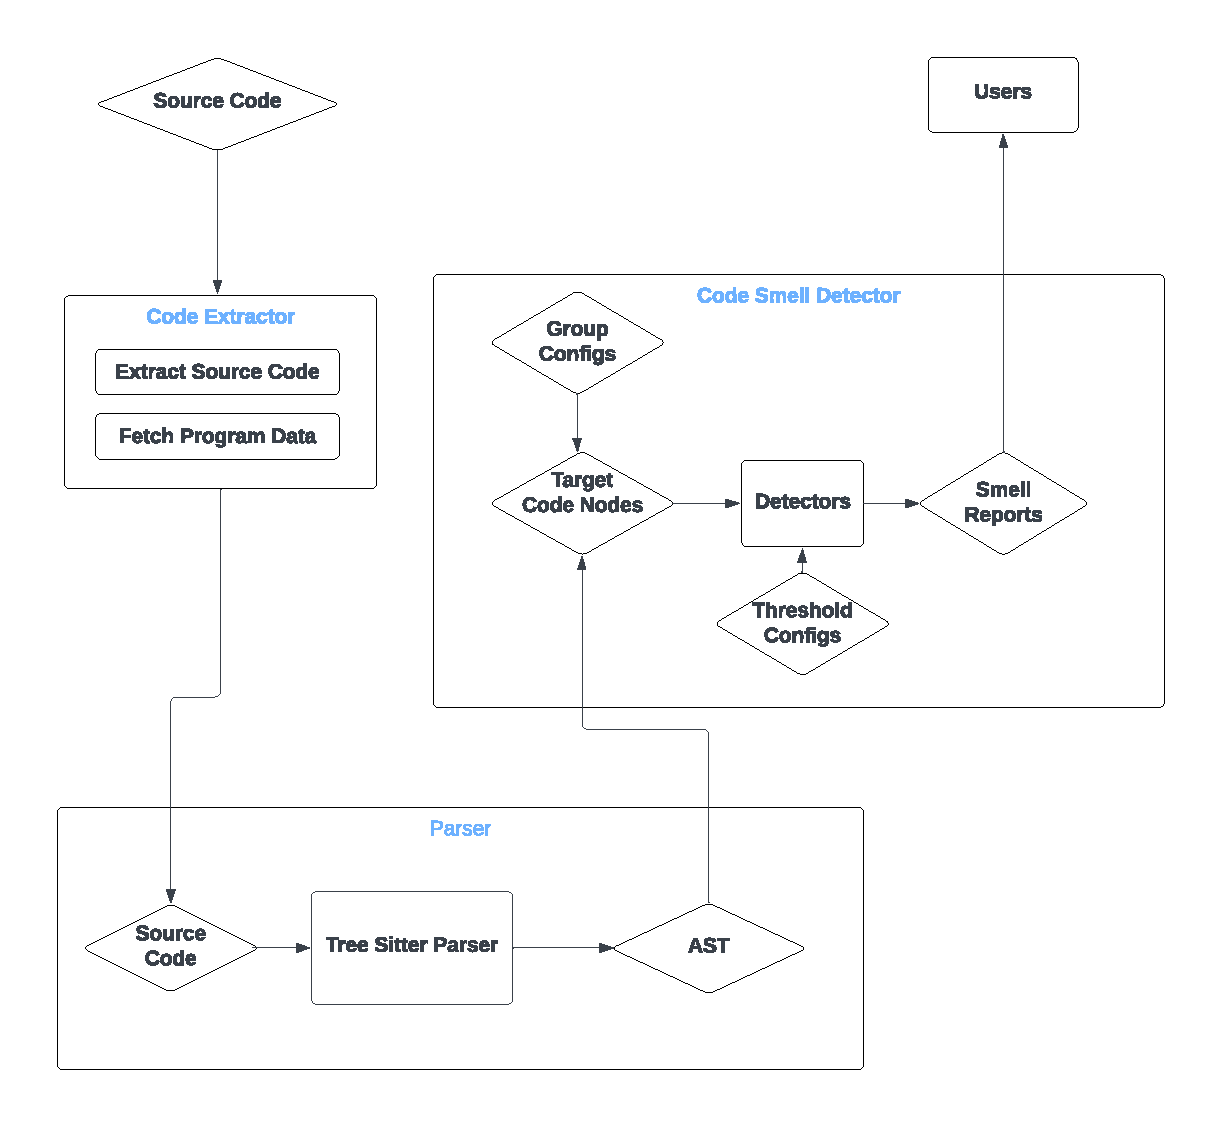
\includegraphics[width=\columnwidth]{graphics/Architecture.pdf}
    %
    \vspace*{-2em}
    %
    \caption{
        % The label should appear _inside_ the caption to ensure
        % Latex numbers it correctly. This is a common gotcha!
        %
        % All figure labels should start with "fig:"
        % So that the figure file can be found easily, the rest of the
        % figure label should be the same as the filename, as it is
        % in this example:
        %
        \label{fig:architecture}
        %
        The TreeNose tool for language-independent code smell detection.
    }
    \vspace*{-1.5em}
    %
    % To save space, you might want to remove space here
    % (use a negative \vspace, e.g. \vspace{-1em})
\end{figure}


\subsection{Detection Procedure}~\label{sec:Detection Procedure}

\texttt{TreeNose} adopts AST-based approach to detect code smells. The
Fig.~\ref{fig:architecture} discloses the architecture of \texttt{TreeNose}.
\texttt{TreeNose} executes 3 steps to detect target code smells. 1. Extract
source code from the project, 2. Parse the source code to AST, 3. Analyze AST
to detect code smells.

\textbf{Step 1: Extract Source Code}: \texttt{TreeNose} recursively extracts
source code matching with the target programming language from the
project. During this procedure, \texttt{TreeNose} fetches all target files
unless the file or the path is in the ignore list.

\textbf{Step 2: Parse Source Code to AST}: \texttt{TreeNose} parses the source
code to AST with Treesitter \cite{treeSitter}. Treesitter is a parser generator
tool that generates AST in multiple programming languages. It currently
supports 18 language bindings. Treesitter decouples the parser from the
language grammar, making it possible to parse the source code in multiple
programming languages.

\textbf{Step 3: Analyze AST to Detect Code Smells}: \texttt{TreeNose} analyzes
AST to detect code smells. Before the analysis, our developers categorize the
language-specific TreeSitter AST nodes like method and function across
programming languages into language-independent groups. This categorization
enables \texttt{TreeNose} to execute the same detection process for nodes in
the same group across multiple programming languages. During the analysis,
\texttt{TreeNose} queries AST and searches for the associated components in
AST. When locating the components, \texttt{TreeNose} calculates the metrics
against the thresholds. Table~\ref{tab:metrics-and-thresholds} shows the
detection metrics with default thresholds for each code smell. Finally,
\texttt{TreeNose} generates reports with the list of code smells detected in
the project.

% Tables should be placed at the top of pages/columns
% where they can.
%
% This can be ensured by using the [t] parameter to the
% "\begin{table}" declaration.
%
\begin{table}[t]
    % Figures should be centered in the page/column
    \centering
    %
    \caption{
        % The label should appear _inside_ the caption to ensure
        % Latex numbers it correctly. This is a common gotcha!
        %
        % All table labels should start with "tab:"
        % So that the figure file can be found easily, the rest of the
        % table's label should be the same as the filename, as it is
        % in this example:
        %
        \label{tab:metrics-and-thresholds}
        %
       Criteria thresholds for identifying smells with TreeNose.
    }
    %
    % Depending on the template, some breathing space might need to
    % be added (use \smallskip \medskip etc.) here
    %
    % Or, to save space, you might want to remove space
    % (use a negative \vspace, e.g. \vspace{-1em})
    %
    %
    % Table content goes here. Use this file to specify the
    % table's column headings. The data should be automatically
    % output from a program processing the raw experimental data
    % and should be inputted from another file. This enables
    % the data to change, if for example, the experiment data
    % needs to be updated.
    %
    % Do not use vertical rules. Ensure you use \toprule, \midrule
    % and \bottomrule from the "booktabs" package effectively.
    %
    % Numbers should be right justified (use "r"),
    % text left justified (use "l").
    %
    % For example:
    %
    \renewcommand{\arraystretch}{1.2}
    \begin{tabular}{@{}lll@{}}
        \toprule
            % use a new line for each column if needed
            {\bf Code Smell}
            &
            {\bf Criteria Threshold}
            &
            {\bf Metrics}
            \\
            %
        \bottomrule
        \input table-data/metrics
    \end{tabular}
    %
    % To save space, you might want to remove space here (use a negative
    % \vspace, e.g. \vspace{-1em})
    \vspace{-1em}
\end{table}

